\section{General Methodology}

\subsection{Process and Sensor Description}

The wall following algorithm implemented follows the process found in
Fig.~\ref{flowch}. 

\begin{figure}[h!]
  \centering \cprotect \fbox{
    \begin{minipage}{3.5in}
      \centering
      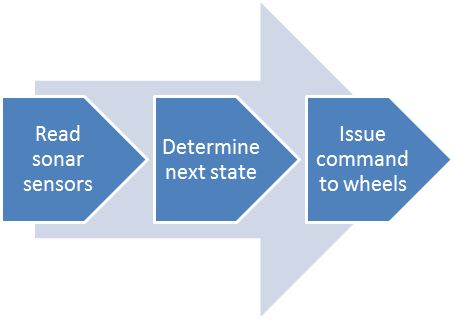
\includegraphics[width =
      \textwidth]{./graphics/flowchart.png}
      \cprotect \caption{Flow chart of wall following algorithm.}
      \label{flowch}
    \end{minipage}
  }
\end{figure}

A switch is used to toggle between following the left wall and
following the right wall. The value of the switch determines which sensors are actively
collecting data. The values of the following sensors will be used:

\begin{itemize}
\item Minimum value of sensors \(s_4\) and \(s_5\) (\(s_0\) and
  \(s_1\) for left-wall following):
  \begin{itemize}
  \item Measure the distance to the closest parallel wall
    (Fig.~\ref{s0s1}).
  \end{itemize}
\item Minimum value of sensors \(s_2\) and \(s_3\):
  \begin{itemize}
  \item Measure the distance to an approaching wall (Fig.~\ref{s2s3}).
  \end{itemize}
\end{itemize}

\begin{figure}[h!]
  \centering \cprotect \fbox{
    \begin{minipage}{3.5in}
      \centering
      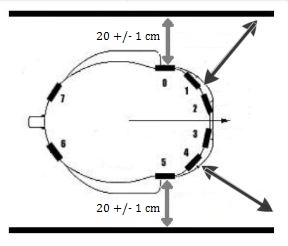
\includegraphics[width =
      \textwidth]{./graphics/s0s1.jpg}
      \cprotect \caption{Sensors \(s_4\) and \(s_5\) (or \(s_0\) and
        \(s_1\)) measuring distance to wall.}
      \label{s0s1}
    \end{minipage}
  }
\end{figure}

\begin{figure}[h!]
  \centering \cprotect \fbox{
    \begin{minipage}{3.5in}
      \centering
      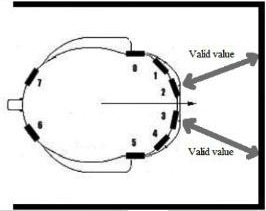
\includegraphics[width =
      \textwidth]{./graphics/s2s3.jpg}
      \cprotect \caption{Sensors \(s_2\) and \(s_3\) 
        measuring distance to front wall.}
      \label{s2s3}
    \end{minipage}
  }
\end{figure}


\subsection{State Machine Description}

The description of the states is listed below. The UML state machine
diagram the team used to implement a solution is found in
Fig.~\ref{state}.

\begin{enumerate}
\item \textbf{Forward:} The robot moves forward alongside a
  wall. A tolerance of \(\pm1\) cm is used to keep the robot in a
  range of 19-21 cm from the wall, measured by sensors
  \(s_4\) and \(s_5\) (or  \(s_0\) and \(s_1\)).  If the distance to the
  wall is not within the specified range, the robot
  switches to one of the adjustment states, which are dependent upon
  which wall is followed.  If a wall is detected in front of the robot
  by sensors \(s_2\) or \(s_3\), the robot switches to the ``inside
  turn'' state. 
\item \textbf{Adjust Outward:} The robot veers slightly outwards to get
  back within the accepted distance range. After the robot is within
  the accepted distance range, the machine switches to the ``forward''
  state.
\item \textbf{Adjust Inward:} The robot veers slightly inwards to get
  back within the accepted distance range. After the robot is within
  the accepted distance range, the machine switches to the ``forward''
  state.
\item \textbf{Inside Turn:} The robot stops and turns \(90^\circ\) clockwise or
  counterclockwise, depending on if the wall followed is on the right
  side or on the left side. Fig.~\ref{it} demonstrates this turn when the
  robot is following a right wall and is turning counterclockwise.
\end{enumerate}

\begin{figure}[h!]
  \centering \cprotect \fbox{
    \begin{minipage}{6.5in}
      \centering
      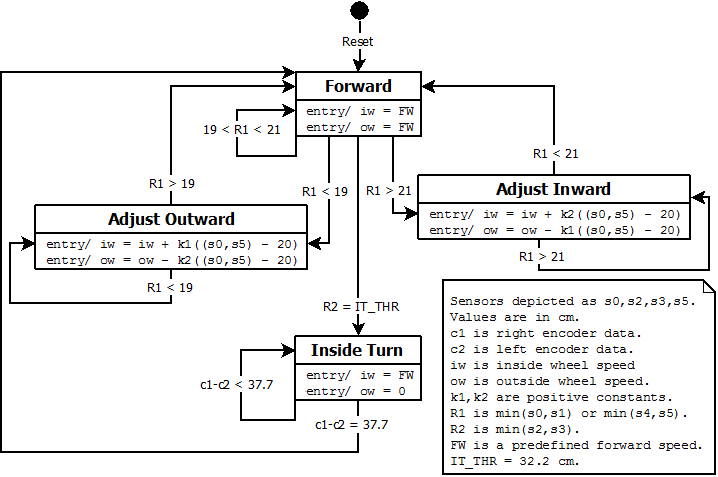
\includegraphics[width =
      \textwidth]{./graphics/smdiagram.png}
      \cprotect \caption{UML state machine diagram for wall following
        algorithm for Amigobot.}
      \label{state}
    \end{minipage}
  }
\end{figure}


\subsection{Navigating Corners}

The robot's turning algorithm takes advantage of the course only
containing turns of approximately 90\(^\circ\). Such sharp turns
are not conducive towards ``smooth'' wall following techniques.
Therefore, when necessary, the robot will execute a blind turn which relies on the
optical rotary encoders on each wheel instead of the sonar data.
The goal of the turning algorithm is not to pivot exactly 90\(^\circ\)
and then move in a straight line every time, but rather to quickly
execute a precise turn which results
in the robot being approximately parallel to and 20 cm away from the
opposite wall, after which the robot can easily continue using sonar
data to make accurate adjustments.

\subsubsection{Detecting a Turn}
The turning algorithm being implemented requires accurate detection of
forward obstacles and discontinuities in the parallel wall in order to
avoid turning prematurely.

The outside turn is not detected directly. Rather, the case of an
absent parallel wall is handled by the ``adjust inward''
state. However, the sensor values for \(s_4\) and \(s_5\) (or \(s_0\)
and \(s_1\)) must be severely limited in order to avoid having the turn 
be executed too sharply. In the program the working value for these
sensors is limited to \verb+0x0140+, or about 32 cm.

\begin{figure}[h!]
  \centering \cprotect \fbox{
    \begin{minipage}{4.5in}
    \centering
    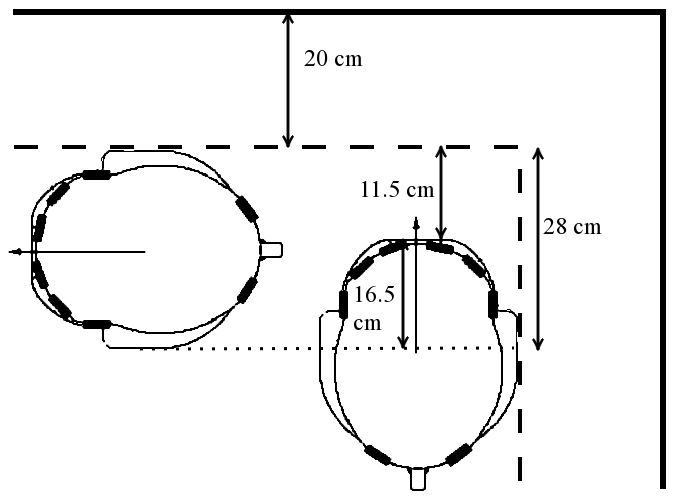
\includegraphics[width =
    \textwidth]{./graphics/inside_turn.png}
    \cprotect \caption{Geometry of an inside turn.}
      \label{it}
    \end{minipage}
  }
\end{figure}

For an inside turn, the robot must begin turning once the front of the
robot reaches the threshold \verb+IT_THR+. The geometry for this turn is
presented in Fig.~\ref{it}, which indicates that \verb+IT_THR+ should
be \(31.5\) cm. However, the forward sensors \(s_2\) and \(s_3\) are
not pointed directly forward, but rather are at \(12^\circ\) angles,
so the sensor reading for \verb+IT_THR+ should be
\(31.5/\cos(12^\circ)=32.2\) cm before the robot begins an inside
turn. The inside turn is executed by stopping the inside wheel while
driving the outside wheel forward until the robot has rotated 90
degrees (see \ref{xturn}). 

\subsubsection{Using Rotary Encoders}

The optical rotary encoders on each wheel of the Amigobot provide an
incredibly fine yet robust way to detect the rotational position of
each wheel. Each wheel's position can be loaded through SCOMP's
I/O through the I/O addresses \verb+0x80+, \verb+0x81+, \verb+0x88+, and
\verb+0x89+, which respectively correspond to the given address names
\verb+LPOSLOW+, \verb+LPOSHIGH+, \verb+RPOSLOW+, and \verb+RPOSHIGH+. The position
datum from each encoder is a 32-bit number. For I/O purposes, this datum
is split into two 16-bit numbers (the upper 16 bits and the lower 16
bits), each of which corresponds to the ``low'' or ``high'' I/O
address for each wheel's position.

\paragraph{Physical Characteristics of the Rotary Encoders}
The encoder datum increments by \(39000\) for each revolution of the
wheel. The left encoder increments when the left wheel is in forward
motion, while the right encoder decrements when the right wheel is in
forward motion. Each wheel has a diameter of 10 cm, which results in a
path of 31.42 cm being traversed for each wheel revolution so long as
traction is maintained. Since there are \(39000\) ``ticks'' per
revolution, one cm of linear wheel motion corresponds to \(1241.41\)
ticks. This results in large-valued encoder data for relatively short
distances. In order to simplify calculations and prevent bit carries
between two 16-bit numbers (the high and low data), it is best to
perform calculations on a single 16-bit number which can be produced
by combining the upper eight bits of the ``low'' datum with the lower
eight bits of the ``high'' datum, resulting in a reduction in encoder
resolution by a factor of 256.  After shifting and truncating the two
16-bit numbers into one 16-bit number, the physical characteristics of
the encoder transform so that there are \(152.34\) ticks per wheel
revolution and \(4.85\) ticks per cm of linear wheel motion.

\subsubsection{Executing a Turn} \label{xturn}
\begin{figure}[h!]
  \centering \cprotect \fbox{
    \begin{minipage}{3.5in}
      \centering
      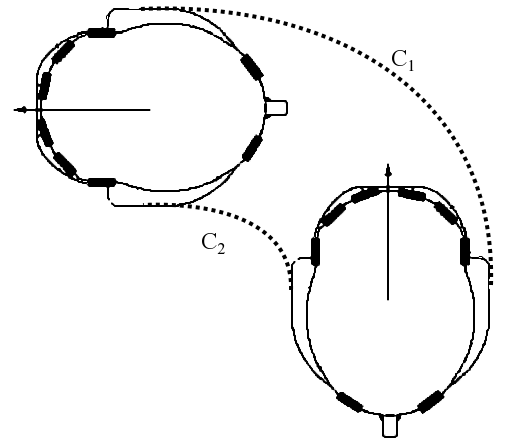
\includegraphics[width = \textwidth]{graphics/turning.png}
      \cprotect \caption{Path lengths \(C_1\) and \(C_2\) as the robot
        turns.}
      \label{turning}
    \end{minipage}
  }
\end{figure}

The linear path lengths of each wheel are related by a constant such
that when the difference in path lengths of each wheel is equal to
that constant, the robot is oriented precisely at an angle \(\theta\)
to its starting orientation. If the robot has a wheel track of \(R\)
and the linear path lengths of the right and left wheels are
represented respectively by \(C_1\) and \(C_2\) (Fig.~\ref{turning}),
then the robot has turned positive (counterclockwise) \(\theta\)
radians when the following equation is satisfied:
\begin{equation}
  C_1 - C_2 = \theta R
\end{equation}
For instance, if the Amigobot (\(R = 24\) cm) is to turn
90\(^\circ\) then continue forward, the robot should cease
turning when \(C_1-C_2 \geq 0.5\pi (24) = 37.7\) cm, or about 181
(\verb+0x00B5+) ticks. Experimentally, it was found that at higher
speeds the wheels of the robot slipped slightly when the robot
decelerated from a turn, so the working
value of this constant was lowered to 154 ticks (\verb+0x009A+).

\subsubsection{Adjustment States}

Once the lateral sensors detect that the robot is outside of the
\(20\pm1\) cm range, the robot enters one of two adjustment
states. The robot feeds back the detected range difference to the left
and right wheel velocities. 

The program uses a cumulative adjustment
where each loop iteration is paused for 100 ms. During each loop
iteration, the angular velocity for each wheel is set to a new value
based on its previous value and the measured distance to the wall, \(R_1\):
\begin{align}
\omega_i [n] &= \omega_i [n -1] + k_1 (R_1 - 20) \label{wi}\\
\omega_o [n] &= \omega_o [n -1] - k_2 (R_1 - 20) \label{wo}
\end{align}
\(\omega_i\) is the inside wheel velocity (right wheel for right-wall
following), \(\omega_o\) is the outside wheel velocity, \(k_1\) and
\(k_2\) are positive constants, and \(R_1\) is the minimum value of sensors \(s_4\)
and \(s_5\) (or \(s_0\) and \(s_1\)).


\subsection{SCOMP Alterations}

Several alterations to the SCOMP program were  made in the form of
new instructions:

\begin{enumerate}
\item \textbf{MULT} - The built-in
  Altera\textregistered~megafunction
  \verb+LPM_MULT+ was implemented into SCOMP, with the module
  multiplying the accumulator, \verb+AC+, and memory data register, \verb+MDR+. The 32-bit result vector
  for \verb+LPM_MULT+ is latched and spread across 16-bit registers
  \verb+LO+ and \verb+HI+ when SCOMP enters the \verb+EX_MULT+
  state. 
\item\textbf{MLO} - The contents of the \verb+LO+ register (the lower
  16 bits of the result of \verb+LPM_MULT+) are
  latched onto the \verb+AC+.
\item \textbf{MHI} - The contents of the \verb+HI+ register (the upper
  16 bits of the result of \verb+LPM_MULT+) are
  latched onto the \verb+AC+.
\item \textbf{DIV} - The megafunction \verb+LPM_DIVIDE+ was
  implemented to divide \verb+AC+ by \verb+MDR+. The remainder of the
  megafunction result is latched onto register \verb+REMAI+.
\item \textbf{REM} - The contents of \verb+REMAI+ are latched onto the
  \verb+AC+. 
\item \textbf{SHIFT2} - The megafunction \verb+LPM_CLSHIFT+ was
  implemented to shift by a variable amount. Instead of the shift
  magnitude being four bits of \verb+IR+ as in the original
  \verb+SHIFT+ instruction, the shift
  amount for \verb+SHIFT2+ is specified by the first four bits of
  \verb+MDR+. Additionally, in order to simplify the assembly program,
  the shift direction was inverted so that when \verb+MDR(4)+ is low,
  a right shift is indicated.
\item \textbf{SHIFT3} - A third instance of megafunction
  \verb+LPM_CLSHIFT+ was implemented in order to provide a variable
  rotating shifter. The megafunction parameters are identical to those
  of \verb+SHIFT2+ except for the shift type. 
\end{enumerate}

The \verb+MULT+, \verb+MHI+, and \verb+MLO+ intructions are used in
the two adjustment states for the multiplication required in equations
\ref{wi} and \ref{wo}. The divide instruction as well as the two shift instructions are used in
manipulating the LED displays as described in section \ref{leds}.

\subsection{Amigobot Display Additions}

Several additions were made to the robot display to improve the user
interface. Memory locations used to write to and read from are designated in capital letters.

\begin{figure}[h!]
  \centering \cprotect \fbox{
    \begin{minipage}{4.5in}
      \centering
      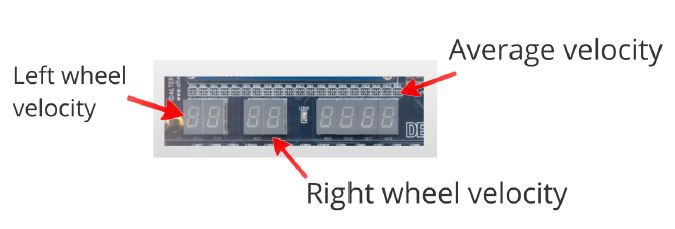
\includegraphics[width = \textwidth]{graphics/7seg.jpg}
      \cprotect \caption{Implementation of both seven-segment
        displays.}
      \label{7seg}
    \end{minipage}
  }
\end{figure}

\begin{itemize}
\item Two displays are used to show the velocity of the left and
  right wheels.
  \begin{itemize}
  \item These are written to \verb+SEVENSEG+ whenever \verb+LVELCMD+
    or \verb+RVELCMD+, the wheel velocities, are changed
    (Fig.~\ref{7seg}).
  \end{itemize}
\item The third display shows the velocity of the robot
  (Fig.~\ref{7seg}).
  \begin{itemize}
  \item This was done by altering the \verb+IO_decoder+ and the block
    diagram files so that the second 7-segment display
    could be written. It is named \verb+SEVENSEG2+ and mapped to
    0x05 on the IO address space map.
  \item\verb+IO_decoder+ was altered by adding and enabling a
    signal for the second set of the 7-segment LEDs and copying the
    setup of the \verb+HEX_DISP+ module used for the current 7-segment
    display.
  \end{itemize}

\begin{figure}[h!]
  \centering \cprotect \fbox{
    \begin{minipage}{4.5in}
      \centering
      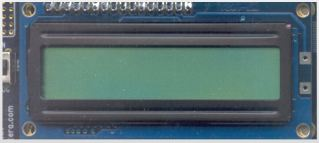
\includegraphics[width = \textwidth]{graphics/lcd.jpg}
      \cprotect \caption{The LCD display on the DE2 board.}
      \label{lcd}
    \end{minipage}
  }
\end{figure}

\item The LCD display (Fig.~\ref{lcd}) shows the current state the program is in.
  \begin{itemize}
  \item This was done by altering the LCD display to accept ASCII
    values representing numbers. The SLCD was altered to take in an
    ASCII enable, \verb+ASCII_EN+, which tells it to interpret the
    incoming argument as a state to be output in ASCII format.
  \item There are four states. The LCD displays \verb+RDY!+ when the
    program is ready to start. It then displays \verb+KEY2+ to tell
    the user to press \verb+KEY2+ and start the program. Once the
    program starts, the screen displays \verb+LEFT+ or \verb+RGHT+,
    telling the user which side of the wall the robot is following.
  \item The states were encoded into a binary code of 16 bits. For
    example, the \verb+RDY!+ output string was encoded as \verb+0x0+ and the
    \verb+KEY2+ command as 0x1. The strings shown on the LCD display
    were hard coded using the binary state representations.
  \end{itemize}

\begin{figure}[h!]
  \centering \cprotect \fbox{
    \begin{minipage}{4.5in}
      \centering
      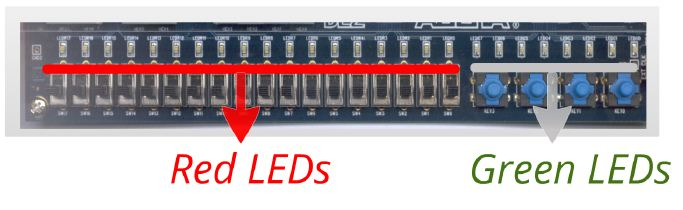
\includegraphics[width = \textwidth]{graphics/ledf.jpg}
      \cprotect \caption{The red and green LED arrays on the DE2
        board.}
      \label{ledf}
    \end{minipage}
  }
\end{figure}

\item The red LEDs (Fig.~\ref{ledf}) light up to show the turning rate
  of the robot.
  \begin{itemize}
  \item Two lit LEDs in the middle (LEDs 7 and 8) form the base
    pattern, which is displayed when the robot is moving in a straight
    line. Otherwise, the displayed pattern is shifted with the
    rotating shifter by an amount proportional to the difference
    between the left and right wheel velocities. This causes the pattern
    to shift left if the robot is turning left, and vice-versa.
  \end{itemize}

\item The green LEDs (Fig.~\ref{ledf}) are used to display a
  completion bar for the ``inside turn'' state.
  \begin{itemize}
  \item This was done by altering \verb+IO_decoder+ and the block
    diagram files so that the green LEDs could be used. It is called
    \verb+GLED+ and mapped to \verb+0x07+ in the IO address space map.
  \end{itemize}
\end{itemize}
\label{leds}

\subsection{Assignments}

\begin{figure}[h!]
  \centering \cprotect \fbox{
    \begin{minipage}{4.5in}
      \centering
      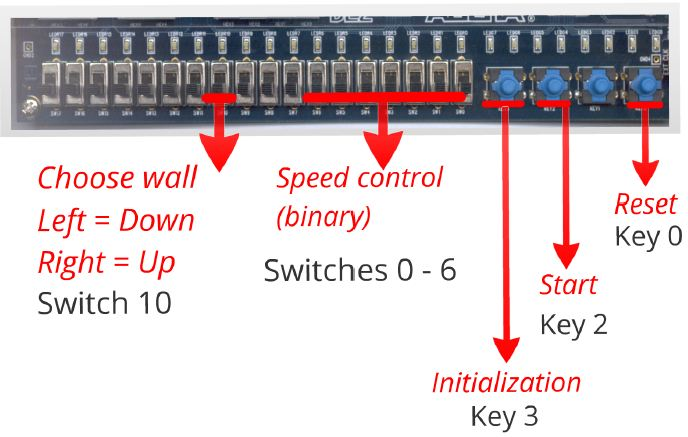
\includegraphics[width = \textwidth]{graphics/assignments.jpg}
      \cprotect \caption{Function assignments for DE2 peripherals.}
      \label{assign}
    \end{minipage}
  }
\end{figure}

The switch and button assignments on the DE2 board are shown in
Fig.~\ref{assign}.  Switches \verb+SW0+ through \verb+SW6+ are used to
encode in binary the speed at which the robot will travel. Switch
\verb+SW10+ selects which wall is to be followed, with a low value
indicating the right-wall following program.
 
To start the program, a series of steps must be followed. First, the
switches are toggled into the desired positions. \verb+KEY3+ is then
pressed to initialize the robot. Lastly, \verb+KEY2+ is pressed to
start the program. \verb+KEY0+ may be pressed at any time to reset
the program.


\subsection{Significant Modifications}

Several significant modifications were made to the original design:

\begin{itemize}
\item The original program consisted of five states. During testing it
  was discovered that the inaccuracy of sensor data when the robot was
  angled to the wall caused premature transitions to an ``outside turn'' state. To
  solve this problem, the state was removed. To navigate outside
  turns, the ``adjust inward'' state is used. A subroutine in this state
  limits the value of the lateral sensors to prevent the robot from
  turning too sharply. 
\item It was originally proposed to use the LCD display to
  show the state that the wall following program is currently
  in. However, since the LCD is not timed on the same clock as
  SCOMP, the team encountered problems timing the latching of IO
  data into the LCD when other IO peripherals,
  such as motor and sensor control, were also being used. To solve
  this problem, the role of  the LCD display was changed to display
  the basic startup states and  not the current wall following  state. 
\item The original design called for one lateral sensor \(s_5\) (or \(s_0\)) and
  one forward sensor \(s_2\) (or \(s_3\)) whose data would serve as inputs to the
  state machine. Since the sensor readings were inaccurate when the
  robot was oriented at an angle to the wall, it was decided that
  using pairs of sensors would be optimal. A pair of sensors, \(s_4\)
  and \(s_5\) (or \(s_0\) and \(s_1\)) was used for the lateral
  region, and the pair \(s_2\) and \(s_3\) for the forward region. The
  minimum value of each pair was used as the working value for the
  distance of the robot to a wall in either the lateral or forward region.
\end{itemize}


\subsection{Project Management}

The finalized Gantt chart that was used during this project can be found in Appendix~\ref{appndx}. 
